\chapter{Química ambiental e toxicologia}\label{ch:b3:environmental-toxicology}

Todo fim de verão, os satélites fotografam redemoinhos verdes que se espalham sobre grandes
lagos: florações de algas alimentadas pelo fosfato e pelo nitrato que escorrem dos campos e
saem das cidades. Quando as algas morrem e afundam, sua decomposição consome o oxigênio da
água profunda, e os peixes morrem. A química explica cada elo dessa cadeia, e de
muitas outras: por que certos gases aquecem o planeta e outros não, por que a chuva é
ácida mesmo em ar limpo, onde um pesticida vai parar depois de pulverizado e quanto
de uma substância é preciso para causar dano. Este capítulo aplica os equilíbrios, a
cinética e a espectroscopia à atmosfera, às águas naturais e aos solos, acompanha os
poluentes entre esses meios e termina com os números sobre os quais se constroem as avaliações de
risco.

\begin{recall}
O volume do 1.º ano tratou dos equilíbrios ácido--base, de precipitação e de complexação,
dos diagramas potencial--pH, dos coeficientes de partição, das meias-vidas, do perigo,
do risco e do sistema GHS; o volume escolar, dos gases de efeito estufa; o volume do 2.º ano,
da lei de Henry, da força iônica, da estatística, da espectrometria de massa e da
espectrometria atômica. O \cref{ch:b3:photochemistry} tratou da fotoquímica atmosférica,
o \cref{ch:b3:group-theory-applied} e o \cref{ch:b3:rovibrational-spectroscopy}, da
atividade no infravermelho, e o \cref{ch:b3:surfaces-catalysis}, da \omterm{def:b3:surfaces-catalysis:adsorption}{adsorção}.
\end{recall}

\begin{omfigure}
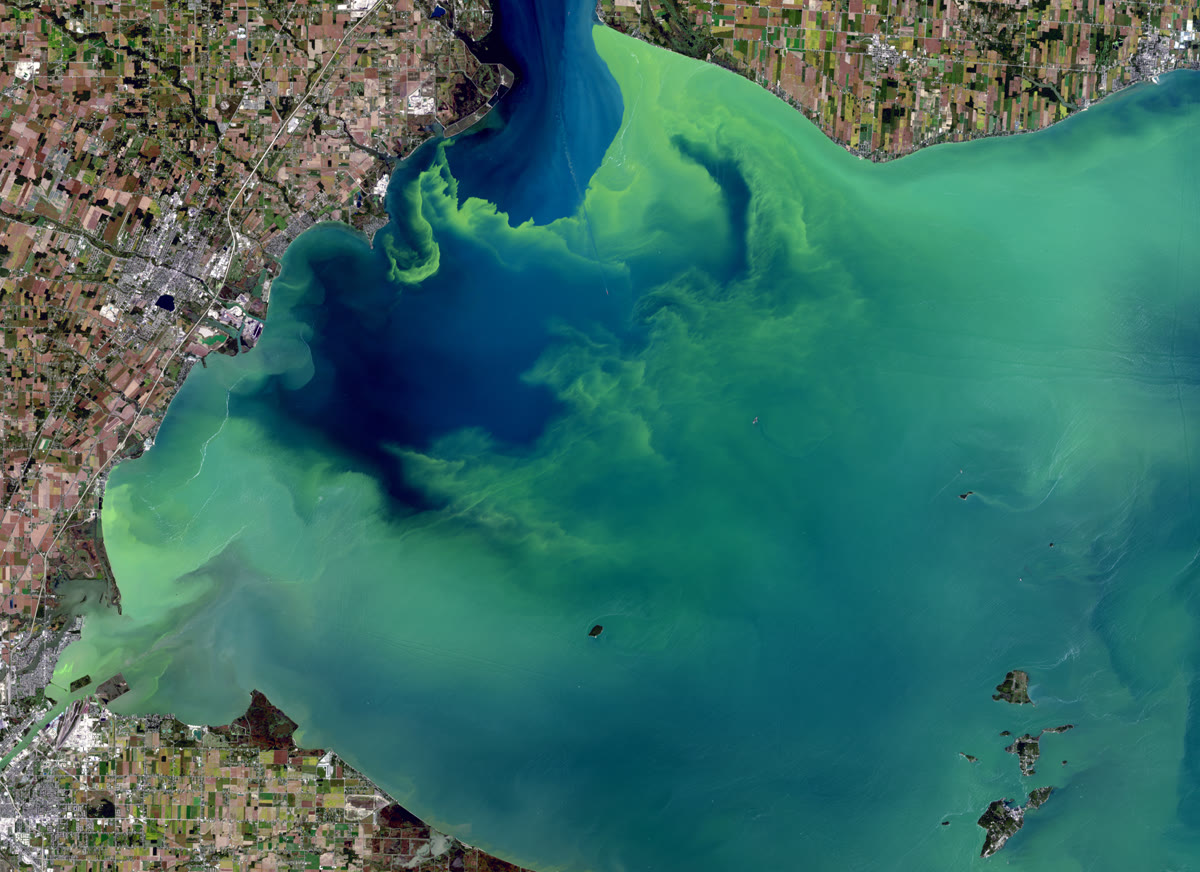
\includegraphics[width=0.62\linewidth]{images/book4/algal-bloom.jpg}

{\small Uma floração de algas em um grande lago, vista por um satélite de observação da Terra no
fim de setembro: os redemoinhos verdes são populações densas de algas microscópicas
alimentadas pelos nutrientes das terras agrícolas vizinhas. Imagem: USGS e NASA, domínio público.}
\end{omfigure}

\section{A atmosfera}

\begin{definition}[Gases de efeito estufa]\label{def:b3:environmental-toxicology:greenhouse}
Um \emph{gás de efeito estufa}\index{gas de efeito estufa@gás de efeito estufa} absorve e emite radiação
infravermelha nos comprimentos de onda da radiação emitida pela superfície da Terra, e
assim aquece a baixa atmosfera. O \emph{potencial de aquecimento
global}\index{potencial de aquecimento global} (GWP) de um gás em um horizonte de tempo,
em geral de 100 anos, é a energia que ele retém após a emissão de um quilograma,
relativa a um quilograma de dióxido de carbono.
\end{definition}

Uma molécula só absorve radiação infravermelha por vibrações que alteram seu
momento dipolar (\cref{ch:b3:group-theory-applied}). O dinitrogênio e o dioxigênio,
diatômicas homonucleares, não têm nenhuma vibração desse tipo e são transparentes; o argônio não tem
vibração alguma. O dióxido de carbono, linear e apolar, tem um modo de deformação angular
ativo no infravermelho perto de \qty{15}{\micro\metre}, no meio da emissão da Terra; a água, o metano
e o óxido nitroso absorvem em muitos comprimentos de onda.

% ledger: atm:CO2.2025, atm:CH4.2025, atm:N2O.2025, gwp:CH4.fossil, gwp:CH4.nonfossil, gwp:N2O, life:CH4, life:N2O
Em 2025, as frações molares médias globais eram de \qty{425.6}{ppm} de dióxido de carbono, \qty{1936}{ppb} de
metano e \qty{338.9}{ppb} de óxido nitroso. O metano, removido pelos radicais hidroxila com um
tempo de vida de cerca de 12 anos, tem um GWP-100 de 27 a 30; o óxido nitroso, destruído apenas na
estratosfera com um tempo de vida de cerca de 109 anos, de 273. O dióxido de carbono não tem
um tempo de vida único: parte de uma emissão permanece no ar por séculos.

\begin{definition}[Poluentes do ar]\label{def:b3:environmental-toxicology:pollutants}
O \emph{material particulado}\index{material particulado} é o conjunto das partículas sólidas e
líquidas em suspensão no ar, classificadas pelo diâmetro aerodinâmico (as partículas finas,
menores que \qty{2.5}{\micro\metre}, penetram fundo nos pulmões). A \emph{chuva
ácida}\index{chuva acida@chuva ácida} é uma chuva tornada mais ácida que a chuva limpa pelos ácidos sulfúrico e
nítrico formados a partir do dióxido de enxofre e dos óxidos de nitrogênio.
\end{definition}

\begin{proposition}[pH da chuva limpa]\label{prop:b3:environmental-toxicology:rain-ph}
A chuva em equilíbrio com o dióxido de carbono do ar atual, e com nada
mais, tem pH de cerca de 5.6.
\end{proposition}

\begin{proof}
% ledger: henry:CO2, pka4:H2CO3.1, pkw4:25C, const:atm
A lei de Henry dá $[\ce{CO2(aq)}] = K_Hp(\ce{CO2}) = \qty{3.4e-7}{mol.L^{-1}.Pa^{-1}} \times (425.6 \times 10^{-6} \times \qty{101325}{Pa}) = \qty{1.47e-5}{mol/L}$. O
balanço de carga é $[\ce{H+}] = [\ce{HCO3-}] + 2[\ce{CO3^2-}] + [\ce{OH-}] \approx K_{a1}[\ce{CO2(aq)}]/[\ce{H+}] + K_w/[\ce{H+}]$, logo
$[\ce{H+}]^2 = K_{a1}[\ce{CO2(aq)}] + K_w = 10^{-6.35} \times \num{1.47e-5} + 10^{-14} = \num{6.6e-12}$: $[\ce{H+}] = \qty{2.6e-6}{mol/L}$, pH 5.6.
\end{proof}

O dióxido de enxofre da queima de combustíveis que contêm enxofre e os óxidos de nitrogênio da
combustão a alta temperatura são oxidados no ar, pelos radicais hidroxila e nas gotículas das
nuvens, a ácidos sulfúrico e nítrico, que levam a chuva a pH 4 e abaixo.
A remoção do enxofre dos combustíveis e dos óxidos de nitrogênio dos gases de escape (conversores
catalíticos, injeção de amônia nas usinas) resolveu em grande parte o problema
onde foi aplicada. O ozônio próximo ao solo, formado quando a luz solar age sobre os
óxidos de nitrogênio e os compostos orgânicos voláteis (\cref{ch:b3:photochemistry}), e
as partículas finas continuam sendo os principais poluentes do ar para a saúde.

\section{Águas naturais}

\begin{omfigure}
\begin{tikzpicture}
\begin{axis}[name=a, width=0.48\linewidth, height=5.4cm, xmin=4, xmax=13, ymin=0, ymax=1.02,
  axis lines=left, xlabel={pH}, ylabel={fração do carbono dissolvido},
  tick label style={font=\scriptsize}, label style={font=\small}]
\addplot[color=omDef, thick] table[x=pH, y=a0] {figdata/out/bachelor-3-carbonate-system.dat};
\addplot[color=omMeth, thick] table[x=pH, y=a1] {figdata/out/bachelor-3-carbonate-system.dat};
\addplot[color=omThm, thick] table[x=pH, y=a2] {figdata/out/bachelor-3-carbonate-system.dat};
\node[font=\scriptsize, omDef] at (axis cs:4.9,0.85) {$\ce{CO2(aq)}$};
\node[font=\scriptsize, omMeth] at (axis cs:8.3,0.88) {$\ce{HCO3-}$};
\node[font=\scriptsize, omThm] at (axis cs:12.1,0.85) {$\ce{CO3^2-}$};
\draw[black!30, dashed] (axis cs:6.35,0) -- (axis cs:6.35,0.5) (axis cs:10.33,0) -- (axis cs:10.33,0.5);
\end{axis}
\begin{axis}[at={(a.east)}, anchor=west, xshift=1.4cm, width=0.48\linewidth, height=5.4cm,
  xmin=0, xmax=2000, ymin=5.2, ymax=6.2, axis lines=left,
  xlabel={$\ce{CO2}$ no ar / ppm}, ylabel={pH da chuva},
  tick label style={font=\scriptsize}, label style={font=\small},
  scaled x ticks=false, xticklabel style={/pgf/number format/1000 sep={}}]
\addplot[color=omDef, thick] table[x=ppm, y=pH] {figdata/out/bachelor-3-carbonate-system-b.dat};
\draw[black!35, dashed] (axis cs:425.6,5.2) -- (axis cs:425.6,5.59);
\node[font=\scriptsize, anchor=west] at (axis cs:470,5.63) {hoje: 5.6};
\end{axis}
\end{tikzpicture}

{\small À esquerda: distribuição do carbono inorgânico dissolvido entre suas três formas
em função do pH a \qty{25}{\celsius}, com cruzamentos em $\mathrm pK_{a1} = 6.35$ e $\mathrm pK_{a2} = 10.33$. À direita: pH da chuva em
equilíbrio apenas com o dióxido de carbono, em função de sua fração molar no ar.}
\end{omfigure}

\begin{proposition}[Frações dos carbonatos]\label{prop:b3:environmental-toxicology:carbonate-fractions}
Com $C_T$ o carbono inorgânico dissolvido total,
$[\ce{CO2(aq)}] = C_Th^2/D$, $[\ce{HCO3-}] = C_TK_{a1}h/D$, $[\ce{CO3^2-}] = C_TK_{a1}K_{a2}/D$, onde $h = [\ce{H+}]$ e $D = h^2 + K_{a1}h + K_{a1}K_{a2}$.
\end{proposition}

\begin{proof}
A partir das duas constantes de acidez,
\[
  [\ce{HCO3-}] = \frac{K_{a1}[\ce{CO2(aq)}]}{h}, \qquad [\ce{CO3^2-}] = \frac{K_{a2}[\ce{HCO3-}]}{h} = \frac{K_{a1}K_{a2}[\ce{CO2(aq)}]}{h^2}.
\]
Sua soma é $C_T = [\ce{CO2(aq)}]\,D/h^2$; dividindo cada forma por $C_T$, obtêm-se as frações.
\end{proof}

\begin{definition}[Alcalinidade]\label{def:b3:environmental-toxicology:alkalinity}
A \emph{alcalinidade}\index{alcalinidade} de uma água é sua capacidade de neutralizar
ácido forte, medida por titulação até o ponto final do ácido carbônico (cerca de pH
4.5) e expressa em mols de $\ce{H+}$ por litro.
\end{definition}

\begin{proposition}[Alcalinidade carbonática]\label{prop:b3:environmental-toxicology:alkalinity}
Em uma água cujas bases são as espécies carbonatadas e o hidróxido,
$\mathrm{Alk} = [\ce{HCO3-}] + 2[\ce{CO3^2-}] + [\ce{OH-}] - [\ce{H+}]$; ela é igual ao excesso das cargas dos cátions de bases fortes
sobre as dos ânions de ácidos fortes e não muda quando o dióxido de carbono
é trocado com o ar.
\end{proposition}

\begin{proof}
A titulação até o ponto final do ácido carbônico transforma todo $\ce{HCO3-}$ em $\ce{CO2}$ (um $\ce{H+}$ cada),
todo $\ce{CO3^2-}$ em $\ce{CO2}$ (dois), todo $\ce{OH-}$ em água (um), enquanto o $\ce{H+}$ livre já presente
conta contra: a soma enunciada. O balanço de carga da água, com
$\ce{Na+}$, $\ce{Ca^2+}$\dots{} e $\ce{Cl-}$, $\ce{SO4^2-}$\dots, se rearranja na mesma soma, igual a $\sum z_i c_i$(cátions) $-$ $\sum z_jc_j$(ânions)
dos eletrólitos fortes. Adicionar ou remover $\ce{CO2}$ não altera nenhum desses íons.
\end{proof}

\begin{definition}[Acidificação dos oceanos]\label{def:b3:environmental-toxicology:acidification}
A \emph{acidificação dos oceanos}\index{acidificacao dos oceanos@acidificação dos oceanos} é a diminuição do
pH da água do mar à medida que ela absorve dióxido de carbono do ar. O \emph{estado de
saturação}\index{estado de saturacao@estado de saturação} de um mineral carbonatado é
$\Omega = [\ce{Ca^2+}][\ce{CO3^2-}]/K_{sp}$: acima de 1, o mineral pode se formar; abaixo de 1, tende a se dissolver.
\end{definition}

O dióxido de carbono dissolvido converte os íons carbonato em hidrogenocarbonato, $\ce{CO2 + CO3^2- + H2O -> 2HCO3-}$,
abaixando o pH e $\Omega$: as conchas e os esqueletos dos corais tornam-se mais difíceis de construir. (Na
água do mar, as constantes são aparentes, medidas no meio salino, e
diferem dos valores em água doce deste capítulo.)

\begin{definition}[Dureza da água]\label{def:b3:environmental-toxicology:hardness}
A \emph{dureza}\index{dureza da agua@dureza da água} de uma água é sua concentração total
de íons cálcio e magnésio, muitas vezes expressa como a massa de carbonato de cálcio
que conteria o mesmo número de mols, em mg/L.
\end{definition}

\begin{definition}[Demanda de oxigênio]\label{def:b3:environmental-toxicology:oxygen-demand}
A \emph{demanda bioquímica de oxigênio}\index{demanda bioquimica de oxigenio@demanda bioquímica de oxigênio} (BOD) de uma
água é a massa de dioxigênio consumida por litro pelos microrganismos que oxidam sua
matéria orgânica no escuro, durante um tempo determinado (cinco dias a \qty{20}{\celsius} para a $\mathrm{BOD_5}$). Sua
\emph{demanda química de oxigênio}\index{demanda quimica de oxigenio@demanda química de oxigênio} (COD) é a massa de
dioxigênio equivalente ao dicromato consumido na oxidação química de sua matéria
orgânica.
\end{definition}

\begin{proposition}[Curva da BOD]\label{prop:b3:environmental-toxicology:bod}
Se a matéria orgânica biodegradável é consumida segundo uma cinética de primeira ordem de constante de
velocidade $k$, o oxigênio usado após um tempo $t$ é $\mathrm{BOD}_t = L_0(1 - \eu^{-kt})$, onde $L_0$ é a BOD final.
\end{proposition}

\begin{proof}
A demanda restante $L$ obedece a $\dd L/\dd t = -kL$, logo $L = L_0\eu^{-kt}$; o oxigênio usado é o que se foi,
$L_0 - L$.
\end{proof}

\begin{omfigure}
\begin{tikzpicture}
\begin{axis}[name=a, width=0.48\linewidth, height=5.2cm, xmin=0, xmax=30, ymin=0, ymax=270,
  axis lines=left, xlabel={tempo / dias}, ylabel={BOD / \unit{mg.L^{-1}}},
  tick label style={font=\scriptsize}, label style={font=\small}]
\addplot[color=omDef, thick] table[x=t, y=bod] {figdata/out/bachelor-3-bod.dat};
\draw[black!35, dashed] (axis cs:0,250) -- (axis cs:30,250);
\draw[black!35, dashed] (axis cs:5,0) -- (axis cs:5,170.8);
\node[font=\scriptsize, anchor=west] at (axis cs:5.6,140) {$\mathrm{BOD_5}$};
\node[font=\scriptsize, anchor=north east] at (axis cs:30,246) {$L_0$};
\end{axis}
\begin{axis}[at={(a.east)}, anchor=west, xshift=1.4cm, width=0.48\linewidth, height=5.2cm,
  xmin=0, xmax=15, ymin=0, ymax=10, axis lines=left,
  xlabel={tempo a jusante / dias}, ylabel={$\ce{O2}$ dissolvido / \unit{mg.L^{-1}}},
  tick label style={font=\scriptsize}, label style={font=\small}]
\addplot[color=omThm, thick] table[x=t, y=O2] {figdata/out/bachelor-3-bod-b.dat};
\draw[black!35, dashed] (axis cs:0,9.1) -- (axis cs:15,9.1);
\node[font=\scriptsize, anchor=south east] at (axis cs:15,9.1) {saturado};
\node[font=\scriptsize, anchor=north] at (axis cs:2.4,6.3) {ponto crítico};
\end{axis}
\end{tikzpicture}

{\small À esquerda: a BOD de um esgoto-modelo, $L_0 = \qty{250}{mg/L}$ e $k = \qty{0.23}{d^{-1}}$: cerca de dois terços da
demanda são consumidos em cinco dias. À direita: a depressão de oxigênio em um rio abaixo de um lançamento
(modelo de Streeter--Phelps): a decomposição da carga orgânica consome oxigênio mais depressa do que
o ar o repõe no início, até que o déficit atinja um máximo após cerca de 2.4 dias.}
\end{omfigure}

\begin{method}[Determinar a COD]\label{met:b3:environmental-toxicology:cod}
\begin{enumerate}
  \item Leve a refluxo um volume medido de amostra com um excesso conhecido de
        dicromato de potássio em ácido sulfúrico, com sulfato de prata como catalisador e
        sulfato de mercúrio(II) para complexar o cloreto.
  \item Titule o dicromato restante com ferro(II) usando ferroína, e faça um
        branco com água pura.
  \item O dicromato consumido, convertido na massa equivalente de $\ce{O2}$ (um
        $\ce{Cr2O7^2-}$ recebe seis elétrons, como fariam 1.5 $\ce{O2}$), dividido pelo volume da amostra, é a
        COD em mg/L.
\end{enumerate}
\end{method}

\begin{definition}[Eutrofização]\label{def:b3:environmental-toxicology:eutrophication}
A \emph{eutrofização}\index{eutrofizacao@eutrofização} é o enriquecimento de um corpo d'água
em nutrientes, sobretudo fósforo e nitrogênio, que leva a um crescimento excessivo de
algas e de plantas, depois ao esgotamento do oxigênio quando elas se decompõem.
\end{definition}

\begin{omfigure}
\begin{tikzpicture}[font=\scriptsize, >=Stealth,
  box/.style={draw, rounded corners, align=center, fill=omMeth!10, inner sep=3pt, minimum height=8mm}]
  \node[box] (f) at (-3.4,1.2) {campos:\\ fertilizantes,\\ esterco};
  \node[box] (t) at (-3.4,-0.4) {cidades: esgoto,\\ detergentes};
  \node[box] (a) at (0,2.1) {atmosfera:\\ deposição (N)};
  \node[box, fill=omDef!12, minimum width=3.2cm, minimum height=1.7cm] (l) at (0.6,0.4) {água do lago:\\ as algas crescem};
  \node[box, fill=black!8] (s) at (0.6,-1.6) {sedimento: P armazenado,\\ liberado em anoxia};
  \node[box] (o) at (4.0,0.4) {efluente};
  \draw[->, thick] (f) -- node[above, sloped, pos=0.4] {\tiny\hspace*{1em}escoamento} (l);
  \draw[->, thick] (t) -- node[below, sloped] {N, P} (l);
  \draw[->, thick] (a) -- (l);
  \draw[->, thick] (l) -- node[left] {algas mortas} (s);
  \draw[->, thick, dashed] (s.east) to[bend right=30] node[right] {P} (l.south east);
  \draw[->, thick] (l) -- (o);
\end{tikzpicture}

{\small Fluxos de nutrientes para um lago e dentro dele. O fósforo, muitas vezes o nutriente
limitante em água doce, acumula-se no sedimento e volta à água
quando o fundo perde seu oxigênio, o que pode sustentar florações durante anos depois que os
aportes são cortados.}
\end{omfigure}

As algas absorvem carbono, nitrogênio e fósforo em proporções aproximadamente constantes;
o nutriente que estiver em falta em relação a essas necessidades limita seu crescimento. Na
maioria dos lagos, é o fósforo, e é por isso que os fosfatos foram retirados dos
detergentes e dos esgotos tratados; em muitos mares costeiros, é o nitrogênio.

\begin{definition}[Especiação]\label{def:b3:environmental-toxicology:speciation}
A \emph{especiação química}\index{especiacao quimica@especiação química} de um elemento em uma
amostra é a distribuição de sua quantidade entre suas formas químicas: estados de
oxidação, complexos, compostos organometálicos, espécies livres e ligadas.
\end{definition}

A toxicidade depende da especiação. O mercúrio inorgânico liberado na água é
metilado por bactérias nos sedimentos em metilmercúrio, que atravessa as membranas,
liga-se ao enxofre das proteínas e se concentra ao longo das cadeias alimentares; o arsênio é muito mais
tóxico como arsenito, As(III), do que como arsenato, As(V), e muito menos nas formas
orgânicas encontradas nos frutos do mar. Uma concentração total, sozinha, diz pouco.

\begin{method}[Especiação de um metal em uma água]\label{met:b3:environmental-toxicology:speciation}
\begin{enumerate}
  \item Liste os ligantes presentes (hidróxido, carbonato, cloreto, sulfato, matéria
        orgânica) com suas concentrações e o pH.
  \item Escreva as constantes de complexação e o balanço de massa do metal, como no
        volume do 1.º ano.
  \item Resolva para o íon metálico livre, depois para cada complexo; trace as frações em função do
        pH ou da concentração de um ligante.
  \item Compare a forma tóxica ou biodisponível (muitas vezes o íon livre) com o total.
\end{enumerate}
\end{method}

\section{Solos e sedimentos}

\begin{definition}[Sorção nos solos]\label{def:b3:environmental-toxicology:soil}
A \emph{capacidade de troca catiônica}\index{capacidade de troca cationica@capacidade de troca catiônica} de um solo é
a quantidade de cátions trocáveis que ele pode reter por unidade de massa, nas argilas e na matéria
orgânica. O \emph{coeficiente de distribuição solo--água}\index{coeficiente de distribuicao solo--agua@coeficiente de distribuição solo--água}
$K_d$ é a razão entre a concentração de uma substância
sorvida no solo (por quilograma) e sua concentração na água dos poros (por
litro); o \emph{coeficiente de partição do carbono orgânico}\index{coeficiente de particao do carbono organico@coeficiente de partição do carbono orgânico}
é $K_{oc} = K_d/f_{oc}$, com $f_{oc}$ a fração mássica de carbono orgânico.
\end{definition}

Os compostos orgânicos neutros se sorvem sobretudo na matéria orgânica do solo, de modo que $K_{oc}$ varia
muito menos de um solo para outro que $K_d$. Um composto com $K_d$ pequeno se desloca com a água
e pode atingir o lençol freático (lixiviação); um com $K_d$ grande permanece perto da superfície,
ligado a partículas que a erosão pode levar para rios e lagos.

\section{Destino dos poluentes}

\begin{definition}[Coeficiente de partição octanol--água]\label{def:b3:environmental-toxicology:kow}
O \emph{coeficiente de partição octanol--água}\index{coeficiente de particao octanol--agua@coeficiente de partição octanol--água}
$K_{ow}$ de uma substância é a razão entre suas concentrações de equilíbrio no
octan-1-ol e na água; ele mede sua afinidade pelos tecidos gordurosos e pela matéria
orgânica.
\end{definition}

% ledger: logkow:DDT, logkow:benzene, logkow:atrazine, logkow:PCB153
O benzeno tem $\log K_{ow} = 2.13$, o herbicida atrazina 2.61, um PCB hexaclorado 6.67 e o
DDT 6.91: os dois últimos se dissolvem na gordura dezenas de milhões de vezes melhor que na
água.

\begin{definition}[Bioacumulação]\label{def:b3:environmental-toxicology:bio}
O \emph{fator de bioconcentração}\index{fator de bioconcentracao@fator de bioconcentração} (BCF) é a
razão entre a concentração em um organismo e a concentração na água ao redor em
estado estacionário, com captação apenas a partir da água. A \emph{bioacumulação}\index{bioacumulacao@bioacumulação}
é o acúmulo em um organismo por todas as vias, inclusive a alimentação;
a \emph{biomagnificação}\index{biomagnificacao@biomagnificação} é o aumento da
concentração da presa ao predador ao longo de uma cadeia alimentar.
\end{definition}

\begin{proposition}[BCF e $K_{ow}$]\label{prop:b3:environmental-toxicology:bcf-kow}
Para as substâncias orgânicas neutras que não são metabolizadas, $\log\mathrm{BCF}$ nos peixes é
aproximadamente uma função linear de $\log K_{ow}$, com inclinação próxima de 1, até $\log K_{ow}$ perto de 6;
acima disso, a captação se torna mais lenta e a relação se estabiliza (regressões empíricas).
\admitted
\end{proposition}

\begin{definition}[Poluentes orgânicos persistentes]\label{def:b3:environmental-toxicology:pop}
Um \emph{poluente orgânico persistente}\index{poluente organico persistente@poluente orgânico persistente} é uma
substância orgânica que resiste à degradação, se bioacumula, é tóxica e é
transportada para longe de suas fontes, como o DDT, os PCBs e as dioxinas.
\end{definition}

\begin{proposition}[Distribuição de equilíbrio entre compartimentos]\label{prop:b3:environmental-toxicology:level-one}
Uma massa $M$ de uma substância distribuída em equilíbrio (um modelo de ``nível I'') entre a água
(volume $V_w$), o ar ($V_a$), os sólidos do sedimento ($m_s$) e os peixes ($m_f$) tem a concentração na água
$C_w = M/(V_w + K_{aw}V_a + K_{sw}m_s + K_{fw}m_f)$, onde os $K$ são os coeficientes de partição em relação à
água; a massa em cada compartimento é seu termo vezes $C_w$.
\end{proposition}

\begin{proof}
No equilíbrio, $C_a = K_{aw}C_w$, $C_s = K_{sw}C_w$ (por quilograma), $C_f = K_{fw}C_w$. O balanço de massa é
$M = C_wV_w + C_aV_a + C_sm_s + C_fm_f = C_w(V_w + K_{aw}V_a + K_{sw}m_s + K_{fw}m_f)$; dividindo, obtém-se $C_w$.
\end{proof}

\begin{omfigure}
\begin{tikzpicture}[font=\scriptsize, >=Stealth,
  comp/.style={draw, rounded corners, align=center, minimum width=2.6cm, minimum height=1.0cm}]
  \node[comp, fill=omDef!8] (air) at (0,2.2) {ar\\ $C_a = K_{aw}C_w$};
  \node[comp, fill=omDef!25] (w) at (0,0.6) {água\\ $C_w$};
  \node[comp, fill=black!10] (sed) at (0,-1.0) {sedimento\\ $C_s = K_{sw}C_w$};
  \node[comp, fill=omMeth!15] (fish) at (3.6,0.6) {peixes\\ $C_f = K_{fw}C_w$};
  \node[comp, fill=omProp!15] (soil) at (-3.6,0.6) {solo\\ $C_{soil} = K_dC_w$};
  \draw[<->, thick] (air) -- (w); \draw[<->, thick] (w) -- (sed);
  \draw[<->, thick] (w) -- (fish); \draw[<->, thick] (w) -- (soil);
\end{tikzpicture}

{\small Compartimentos de um modelo de equilíbrio (nível I): cada compartimento está em
equilíbrio com a água, e sua concentração é fixada por um coeficiente de partição.
A substância se acumula onde o produto da capacidade pelo volume (ou pela massa) é
maior, muitas vezes o sedimento ou o solo para um composto hidrofóbico.}
\end{omfigure}

\section{Toxicologia e regulamentação}

\begin{definition}[Dose--resposta]\label{def:b3:environmental-toxicology:dose}
Uma \emph{relação dose--resposta}\index{relacao dose--resposta@relação dose--resposta} liga
a dose de uma substância à intensidade ou à frequência de um efeito. A \emph{dose letal
mediana}\index{dose letal mediana} $\mathrm{LD_{50}}$ mata metade de uma população de teste; a
\emph{concentração efetiva mediana}\index{concentracao efetiva mediana@concentração efetiva mediana} $\mathrm{EC_{50}}$
causa um efeito determinado em metade dela. O \emph{nível sem efeito adverso
observado}\index{nivel sem efeito adverso observado@nível sem efeito adverso observado} (NOAEL) é a maior dose testada
sem efeito adverso; o \emph{menor nível com efeito adverso
observado}\index{menor nivel com efeito adverso observado@menor nível com efeito adverso observado} (LOAEL), a menor dose testada
com efeito adverso.
\end{definition}

\begin{proposition}[Modelo log-logístico]\label{prop:b3:environmental-toxicology:dose-response}
No modelo log-logístico $f(d) = 1/\bigl(1 + (D_{50}/d)^n\bigr)$, a resposta vale um meio em $d = D_{50}$, e $n$
mede a inclinação: a razão de doses entre as respostas de 10\,\% e de 90\,\% é $81^{1/n}$.
\end{proposition}

\begin{proof}
Em $d = D_{50}$, $f = 1/2$. $f = 0.1$ exige $(D_{50}/d)^n = 9$, $f = 0.9$ exige $(D_{50}/d)^n = 1/9$; a razão entre as duas doses
é $(9 \times 9)^{1/n} = 81^{1/n}$.
\end{proof}

\begin{omfigure}
\begin{tikzpicture}
\begin{axis}[width=0.72\linewidth, height=5.4cm, xmode=log, xmin=3, xmax=3200, ymin=0, ymax=1.02,
  axis lines=left, xlabel={dose / \unit{mg.kg^{-1}}}, ylabel={fração que responde},
  tick label style={font=\scriptsize}, label style={font=\small}]
\addplot[color=omDef, thick] table[x=d, y=n2] {figdata/out/bachelor-3-dose-response.dat};
\addplot[color=omThm, thick] table[x=d, y=n6] {figdata/out/bachelor-3-dose-response.dat};
\addplot[only marks, mark=*, mark size=1.6pt, omThm] table[x=d, y=r] {figdata/out/bachelor-3-dose-response-b.dat};
\draw[black!35, dashed] (axis cs:200,0) -- (axis cs:200,0.5) -- (axis cs:3,0.5);
\node[font=\scriptsize, anchor=north west] at (axis cs:200,0.48) {$D_{50}$};
\node[font=\scriptsize, omThm, anchor=south east, inner sep=1pt] (noael) at (axis cs:60,0.09) {NOAEL};
\draw[omThm] (noael.south east) -- (axis cs:78,0.012);
\node[font=\scriptsize, omThm, anchor=west] at (axis cs:165,0.2) {LOAEL};
\node[font=\scriptsize, omDef, anchor=east] at (axis cs:60,0.25) {$n = 2$};
\node[font=\scriptsize, omThm, anchor=east] at (axis cs:185,0.8) {$n = 6$};
\end{axis}
\end{tikzpicture}

{\small Curvas dose--resposta log-logísticas com a mesma dose mediana (\qty{200}{mg/kg},
modelo) e duas inclinações. Os pontos são um estudo com cinco doses para a curva mais
íngreme: com uma resposta de 5\,\% como critério de efeito adverso, o NOAEL é
\qty{80}{mg/kg} e o LOAEL, \qty{160}{mg/kg}; ambos dependem das doses escolhidas.}
\end{omfigure}

\begin{definition}[Toxicidade aguda e crônica]\label{def:b3:environmental-toxicology:toxicity}
A \emph{toxicidade aguda}\index{toxicidade aguda} é o dano causado por uma única
exposição ou por exposições em um curto intervalo; a \emph{toxicidade crônica}\index{toxicidade cronica@toxicidade crônica},
o causado por uma exposição repetida ou contínua durante uma longa parte da vida.
\end{definition}

% ledger: ld50:NaCl, ld50:caffeine, ld50:nicotine
A toxicidade é uma questão de dose: a $\mathrm{LD_{50}}$ oral em ratos é de cerca de \qty{3000}{mg/kg} para o cloreto de sódio,
\qty{192}{mg/kg} para a cafeína e \qty{188}{mg/kg} para a nicotina no mesmo tipo de registro. Para a maioria dos efeitos, existe uma
dose limiar abaixo da qual o organismo dá conta; para os carcinógenos genotóxicos,
não se supõe nenhuma, e a exposição é mantida tão baixa quanto razoavelmente possível.

\begin{definition}[Ecotoxicologia]\label{def:b3:environmental-toxicology:ecotoxicology}
A \emph{ecotoxicologia}\index{ecotoxicologia} estuda os efeitos das substâncias sobre os
organismos nos ecossistemas. A \emph{concentração prevista sem
efeito}\index{concentracao prevista sem efeito@concentração prevista sem efeito} (PNEC) é a menor
concentração com efeito ou sem efeito obtida em testes com espécies representativas,
dividida por um fator de avaliação que cobre a incerteza; a
\emph{concentração ambiental prevista}\index{concentracao ambiental prevista@concentração ambiental prevista}
(PEC) é a concentração esperada a partir dos usos e do destino da
substância; o \emph{quociente de risco}\index{quociente de risco} é PEC/PNEC.
\end{definition}

\begin{proposition}[Quociente de risco]\label{prop:b3:environmental-toxicology:risk-quotient}
Um \omterm{def:b3:environmental-toxicology:ecotoxicology}{quociente de risco} menor que 1 não indica preocupação para o compartimento avaliado; acima
de 1, indica um risco que exige dados refinados ou medidas para reduzir a exposição.
\end{proposition}

\begin{proof}[Por definição]
A PNEC é fixada, por meio de seu fator de avaliação, abaixo das concentrações nas quais
se observaram efeitos; uma concentração esperada abaixo dela não deve, portanto,
causar efeitos, e acima dela, sim.
\end{proof}

\begin{method}[Uma avaliação de risco ambiental]\label{met:b3:environmental-toxicology:risk}
\begin{enumerate}
  \item Perigo: reúna os dados de toxicidade para algas, invertebrados e peixes ($\mathrm{EC_{50}}$
        aguda, NOEC crônica); tome o menor; divida pelo fator de avaliação (maior quando
        só existem dados agudos) para obter a PNEC.
  \item Exposição: a partir das quantidades usadas e do destino (partição, degradação),
        calcule a PEC em cada compartimento, ou meça-a.
  \item Risco: calcule PEC/PNEC; se for maior que 1, refine os dados ou reduza a
        exposição, e repita.
\end{enumerate}
\end{method}

\begin{definition}[Limite de exposição ocupacional]\label{def:b3:environmental-toxicology:oel}
Um \emph{limite de exposição ocupacional}\index{limite de exposicao ocupacional@limite de exposição ocupacional} é a
concentração de uma substância no ar de um local de trabalho que os trabalhadores podem respirar,
em média ao longo de uma jornada de trabalho (ou de 15 minutos para os limites de curta duração), sem
efeitos adversos esperados.
\end{definition}

Os novos produtos químicos colocados no mercado em quantidade precisam ser registrados com um
dossiê de suas propriedades, perigos e usos; os mais perigosos podem ser
restringidos ou permitidos apenas para usos autorizados.

\begin{inthelab}[Medir a $\mathrm{BOD_5}$]
Uma amostra é diluída com água de diluição aerada contendo nutrientes e um
inóculo bacteriano, de modo que boa parte, mas não todo, o oxigênio seja consumido. Dois
frascos com tampa são enchidos até a borda: o oxigênio dissolvido de um é medido
imediatamente com um eletrodo de oxigênio, o do outro após cinco dias no escuro a
\qty{20}{\celsius}. A diferença, multiplicada pelo fator de diluição e corrigida pelo inóculo, é a
$\mathrm{BOD_5}$.
\end{inthelab}

\begin{safety}{\ghs[0.62cm]{GHS03}\ghs[0.62cm]{GHS05}\ghs[0.62cm]{GHS06}\ghs[0.62cm]{GHS08}\ghs[0.62cm]{GHS09}}
% ledger: ghs:K2Cr2O7, ghs4:HgSO4
Os reagentes da COD: o dicromato de potássio é oxidante, pode provocar câncer e
defeitos genéticos, é corrosivo e sensibilizante; o sulfato de mercúrio(II) é fatal se
ingerido, inalado ou em contato com a pele e muito tóxico para os organismos aquáticos. Ambos são
usados em tubos selados, e os tubos usados vão para os resíduos perigosos.
\end{safety}

\begin{history}[Um livro e uma baía]
Em 1962, \textit{Silent Spring} (\textit{Primavera silenciosa}), de Rachel Carson, descreveu o declínio das aves envenenadas pelo
DDT e por outros pesticidas concentrados ao longo das cadeias alimentares, e lançou a regulamentação
ambiental moderna. Alguns anos antes, em 1956, uma doença do sistema
nervoso foi reconhecida entre os habitantes da baía de Minamata: uma fábrica química havia
despejado metilmercúrio, formado a partir de seu catalisador de mercúrio, que se acumulou
nos peixes que os habitantes comiam.
\end{history}

\section{Exercícios}

\begin{exercise}[$\star$]\label{exo:b3:environmental-toxicology:1}
Por que $\ce{N2}$, $\ce{O2}$ e Ar não absorvem no infravermelho, e que vibração do $\ce{CO2}$ faz dele um
\omterm{def:b3:environmental-toxicology:greenhouse}{gás de efeito estufa}?
\end{exercise}

\begin{exercise}[$\star$]\label{exo:b3:environmental-toxicology:2}
Por que fator $[\ce{H+}]$ muda quando o pH da água do mar cai 0.1?
\end{exercise}

\begin{exercise}[$\star$]\label{exo:b3:environmental-toxicology:3}
Uma água contém \qty{2.0}{mmol/L} de $\ce{Ca^2+}$ e \qty{0.50}{mmol/L} de $\ce{Mg^2+}$. Dê sua \omterm{def:b3:environmental-toxicology:hardness}{dureza} em mg de $\ce{CaCO3}$ por litro.
\end{exercise}

\begin{exercise}[$\star$]\label{exo:b3:environmental-toxicology:4}
As algas absorvem C, N e P na razão molar $106 : 16 : 1$ (dados do exercício). Uma água de lago
tem \qty{0.60}{mg/L} de nitrogênio de nitrato e \qty{0.010}{mg/L} de fósforo de fosfato. Que nutriente limita
o crescimento?
\end{exercise}

\begin{exercise}[$\star\star$]\label{exo:b3:environmental-toxicology:5}
Mede-se uma $\mathrm{BOD_5}$ de \qty{170}{mg/L} em um esgoto com $k = \qty{0.23}{d^{-1}}$. Estime sua BOD final.
\end{exercise}

\begin{exercise}[$\star\star$]\label{exo:b3:environmental-toxicology:6}
Uma amostra de água de \qty{100.0}{mL} precisa de \qty{4.40}{mL} de ácido clorídrico \qty{0.0200}{mol/L} para chegar a pH 4.5. Calcule sua
\omterm{def:b3:environmental-toxicology:alkalinity}{alcalinidade} e, supondo que seja toda devida ao hidrogenocarbonato, a concentração deste em mg/L.
\end{exercise}

\begin{exercise}[$\star\star$]\label{exo:b3:environmental-toxicology:7}
Um solo tem $f_{oc} = 0.020$; um pesticida tem $K_{oc} = \qty{300}{L/kg}$ (dados do exercício). Calcule $K_d$ e a
fração do pesticida sorvida em um solo com \qty{1.5}{kg} de sólido por \qty{0.30}{L} de água nos poros.
\end{exercise}

\begin{exercise}[$\star\star$]\label{exo:b3:environmental-toxicology:8}
Com $\log\mathrm{BCF} = 0.85\log K_{ow} - 0.70$ (uma regressão empírica, dados do exercício), estime o BCF do
benzeno e de um PCB hexaclorado, e comente.
\end{exercise}

\begin{exercise}[$\star\star$]\label{exo:b3:environmental-toxicology:9}
Exprima a $\mathrm{LD_{50}}$ oral da cafeína em ratos como uma massa para um adulto de \qty{70}{kg} e como xícaras de café de
\qty{90}{mg} cada (uma extrapolação ingênua, dados do exercício). Por que essa extrapolação é apenas indicativa?
\end{exercise}

\begin{exercise}[$\star\star\star$]\label{exo:b3:environmental-toxicology:10}
Uma substância tem uma $\mathrm{EC_{50}}$ em 48 horas de \qty{0.50}{mg/L} para dáfnias, uma $\mathrm{EC_{50}}$ em 72 horas de \qty{1.2}{mg/L} para algas
e uma $\mathrm{LC_{50}}$ em 96 horas de \qty{2.0}{mg/L} para peixes, todas agudas, e aplica-se um fator de avaliação de 1000
(dados do exercício). Calcule a PNEC e o \omterm{def:b3:environmental-toxicology:ecotoxicology}{quociente de risco} para uma PEC de \qty{0.20}{\micro g/L}.
\end{exercise}

\begin{exercise}[$\star\star\star$]\label{exo:b3:environmental-toxicology:11}
Uma ave piscívora come peixes com \qty{0.30}{mg/kg} de um poluente persistente; os peixes comem
plâncton com \qty{0.015}{mg/kg}; a água contém \qty{2.0}{ng/L}. Calcule os \omterm{def:b3:environmental-toxicology:bio}{fatores de bioconcentração} e de
\omterm{def:b3:environmental-toxicology:bio}{biomagnificação} ao longo da cadeia, se a gordura da ave contém \qty{6.0}{mg/kg} (dados do
exercício).
\end{exercise}

\begin{exercise}[$\star\star\star$]\label{exo:b3:environmental-toxicology:12}
Uma usina emite \qty{1000}{t} de $\ce{SO2}$ por ano. Calcule a massa de ácido sulfúrico que ela pode formar
e o volume de chuva que ela levaria a pH 4.0 se tudo caísse na chuva (despreze os outros
ácidos e bases).
\end{exercise}

\section{Problema: Um pesticida em um lago}

\begin{problem}[{Problema de fim de semana --- um pesticida em um lago: sua partição entre o
sedimento e os peixes, um balanço de massa de equilíbrio, sua degradação ao longo de um ano
e o quociente de risco para os organismos do lago}]
\label{pb:b3:environmental-toxicology:1}
Dados do problema. Um lago contém $\qty{1.0e9}{L}$ de água sob $\qty{1.0e12}{L}$ de ar (a camada de mistura acima dele),
com $\qty{1.0e8}{kg}$ de sólidos ativos do sedimento ($f_{oc} = 0.040$) e $\qty{1.0e4}{kg}$ de peixes (fração lipídica 0.048).
Um pesticida tem $\log K_{ow} = 4.0$, um coeficiente de partição ar--água $K_{aw} = \num{1.0e-4}$ e $K_{oc} = 0.41\,K_{ow}$;
$K_{fw}$ = fração lipídica $\times K_{ow}$. Chegam ao lago 100 kg dele. Sua meia-vida no lago é de 60 dias.
O teste crônico mais sensível dá uma NOEC de \qty{50}{\micro g/L}, com um fator de avaliação de 10;
os peixes para consumo humano não devem exceder \qty{1.0}{mg/kg}.

\medskip\noindent\textbf{Parte I --- Coeficientes de partição.}
\begin{enumerate}
  \item O que $\log K_{ow} = 4.0$ diz sobre o pesticida?
  \item Calcule $K_{oc}$ e o coeficiente sedimento--água $K_{sw}$.
  \item Calcule o coeficiente peixe--água $K_{fw}$.
  \item O pesticida é volátil a partir da água? Use $K_{aw}$.
  \item Por que o carbono orgânico, e não a matéria mineral, governa sua sorção?
  \item Que compartimento você espera que contenha a maior parte dele?
\end{enumerate}

\medskip\noindent\textbf{Parte II --- Balanço de massa de equilíbrio.}
\begin{enumerate}[resume]
  \item Calcule os termos de capacidade $V_w$, $K_{aw}V_a$, $K_{sw}m_s$ e $K_{fw}m_f$.
  \item Calcule a concentração na água.
  \item Calcule a massa em cada compartimento.
  \item Calcule as concentrações no ar, no sedimento e nos peixes.
  \item Que hipótese do modelo é a menos realista?
  \item Como a degradação mudaria o quadro (modelos de nível II e III)?
\end{enumerate}

\medskip\noindent\textbf{Parte III --- Degradação.}
\begin{enumerate}[resume]
  \item Calcule a constante de velocidade de primeira ordem.
  \item Calcule a fração restante após um ano.
  \item Calcule a concentração na água após um ano.
  \item Por que o sedimento pode reter o pesticida por mais tempo do que a meia-vida sugere?
  \item O que torna um pesticida persistente?
\end{enumerate}

\medskip\noindent\textbf{Parte IV --- Risco.}
\begin{enumerate}[resume]
  \item Calcule a PNEC.
  \item Tome a concentração inicial na água como PEC: calcule o \omterm{def:b3:environmental-toxicology:ecotoxicology}{quociente de risco}.
  \item Conclua para os organismos do lago.
  \item Compare a concentração nos peixes com o limite de consumo.
  \item O que você mediria em seguida, e onde?
  \item Que medidas abaixariam a PEC?
  \item Por que o fator de avaliação importa tanto?
  \item Enuncie o resultado: o \omterm{def:b3:environmental-toxicology:ecotoxicology}{quociente de risco} PEC/PNEC.
\end{enumerate}
\end{problem}
